\chapter{Аналитический обзор}
\label{cha:analysis}
%
% % В начале раздела  можно напомнить его цель
%
%В данном разделе анализируется и классифицируется существующая всячина и пути создания новой всячины. А вот отступ справа в 1 см. "--- это хоть и по ГОСТ, но ведь диагноз же...

%%%%%%%%%%%%%%%%%%%%%%%%%%%%%%%%%%%%%%%%%%%%%%%%%%%%%%%%%%%%%%%%%%%%%%%%%%%%%%%%%%%%%%%%%%%%%%%%%%%%%%%%%%%%%%%%

\section{Что такое Интернет вещей}

Интернет вещей (англ. \textit{IoT}, \textit{Internet of Things}) ""--- это методология вычислительной сети физических объектов (``\textit{вещей}''), имеющих встроенную поддержку технологий передачи данных для их взаимодействия, а также для взаимодействия с внешней средой.
Эта методология рассматривает Интернет вещей как явление, способное перестроить культурные и экономические процессы, всё больше исключая человека из них.
Влияние существующего Интернета на сферы образования, коммуникации, бизнеса, науки и политики позволяет говорить о том, что Интернет является одним из важнейших и мощнейших изобретений в истории человечества\cite{evans2011internet}.
Интернет вещей стоит рассматривать как новую ветвь эволюции Интернета, где каждый предмет в поле зрения человека может быть оснащён датчиками, сенсорами, устройством управления и модулем передачи данных для общения со всем миром.

Как известно, большинство великих изобретений человечества потребовали десятки и даже сотни лет на переход от простых по форме представлений до сложных систем.
От создания предпосылок, до массового внедрения Интернета ушло почти четверть века, однако похоже что для Интернета вещей на то же самое потребуется существенно меньше времени \cite{chernyak2013}.
Международный союз связи (МСЭ) и Европейский Союз определили Интернету вещей главенствующую роль в дальнейшем развитии отрасли инфокоммуникации. 
По расчетам консалтингового подразделения Cisco IBSG (см. рис. \ref{fig:iotandpeople}) в промежутке между 2008 и 2009 годами, количество устройств, подключенных к интернету, превысило количество людей, и к 2020 году количество подключенных устройств	достигнет 50 миллиардов\cite{evans2011internet}.
Таким образом, в настоящее время происходит переход от ``Интернета людей'' к ``Интернету вещей''.
Хотя данная концепция на международном уровне уже обретает черты сформировавшейся технологии, для неё ведутся активные работы в области стандартизации компонентов, архитектуры и приложений.
Количество мнений о том как будет построен Интернет вещей очень велико. 
Это подтверждается большим разнообразием предлагаемых технологий для создания LPWAN сетей на рынке.

\begin{figure}
  \centering
  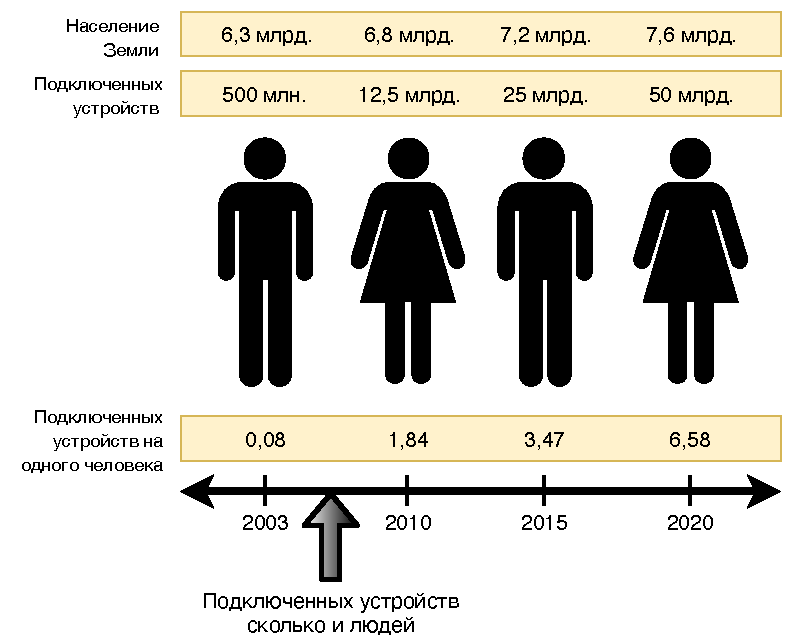
\includegraphics[width=0.7\textwidth]{inc/img/IoTAndPeople}
	\caption{Временная шкала изменения количества людей и предметов, подключенных к интернет \cite{evans2011internet}}
  \label{fig:iotandpeople}
\end{figure}

%Кстати, про картинки. Во-первых, для фигур следует использовать \texttt{[ht]}. Если и после этого картинки вставляются <<не по ГОСТ>>, т.е. слишком далеко от места ссылки, "--- значит у вас в РПЗ \textbf{слишком мало текста}! Хотя и ужасный параметр \texttt{!ht} у окружения \texttt{figure} тоже никто не отменял, только при его использовании документ получается страшный, как в ворде, поэтому просьба так не делать по возможности.

\subsection{Базовые принципы Интернета вещей}

Интернет вещей основывается на трёх базовых принципах\cite{roslyakov2014}.
\begin{enumerate}
	\item повсеместно распространенная инфраструктура;
	\item глобальная идентификация каждого объекта;
	\item возможность каждого физического объекта отправлять и получать данные, посредством локальной сети или сети Интернет, к которой он подключен.
\end{enumerate}

Наиболее важными отличиями Интернета вещей от интернета людей являются:
\begin{itemize}
	\item фокус на считывание информации, а не на коммуникациях;
	\item на порядки большее число подключенных к сети объектов;
	\item потребность в создании новых стандартов;
	\item намного меньше размеры объектов и скорости передачи данных;
	\item фокус не на человеке, а на вещах;
\end{itemize}

%%%%%%%%%%%%%%%%%%%%%%%%%%%%%%%%%%%%%%%%%%%%%%%%%%%%%%%%%%%%%%%%%%%%%%%%%%%%%%%%%%%%%%%%%%%%%%%%%%%%%%%%%%%%%%%%

\section{Обзор технологии LoRa} 

Здесь я обозреваю технологию...

%%%%%%%%%%%%%%%%%%%%%%%%%%%%%%%%%%%%%%%%%%%%%%%%%%%%%%%%%%%%%%%%%%%%%%%%%%%%%%%%%%%%%%%%%%%%%%%%%%%%%%%%%%%%%%%%

\section{Примеры применения технологии LoRa в концепции Интернета вещей}

\subsection{Умный светильник}

\subsection{Умный счётчик}

%%%%%%%%%%%%%%%%%%%%%%%%%%%%%%%%%%%%%%%%%%%%%%%%%%%%%%%%%%%%%%%%%%%%%%%%%%%%%%%%%%%%%%%%%%%%%%%%%%%%%%%%%%%%%%%%

\section{Преимущества и недостатки в сравнении с другими технологиями}

\subsection{Sigfox}

\subsection{XNB (Стриж)}

\subsection{NB-Fi}

\subsection{LTE/UMTS/GSM}

%Теперь мы покажем, как изменить нумерацию на «нормальную», если вам этого захочется. Пара команд в начале документа поможет нам.

%\renewcommand{\labelenumi}{\arabic{enumi})}
%\renewcommand{\labelenumii}{\asbuk{enumii})}

%\begin{enumerate}
%\item Изменим нумерацию на более привычную...
%\item ... нарушим этим гост.
%\begin{enumerate}
%\item Но, пожалуй, так лучше.
%\end{enumerate}
%\end{enumerate}

%В заключение покажем произвольные маркеры в списках. Для них нужен пакет \textbf{enumerate}.
%\begin{enumerate}[1.]
%\item Маркер с арабской цифрой и с точкой.
%\item Маркер с арабской цифрой и с точкой.
%\begin{enumerate}[I.]
%\item Римская цифра с точкой.
%\item Римская цифра с точкой.
%\end{enumerate}
%\end{enumerate}

%В отчётах могут быть и таблицы "--- см. табл.~\ref{tab:tabular} и~\ref{tab:longtable}.
%Небольшая таблица делается при помощи \Code{tabular} внутри \Code{table} (последний
%полностью аналогичен \Code{figure}, но добавляет другую подпись).

%\begin{table}[ht]
  %\caption{Пример короткой таблицы с коротким названием}
  %\begin{tabular}{|r|c|c|c|l|}
  %\hline
  %Тело      & $F$ & $V$  & $E$ & $F+V-E-2$ \\
  %\hline
  %Тетраэдр  & 4   & 4    & 6   & 0         \\
  %Куб       & 6   & 8    & 12  & 0         \\
  %Октаэдр   & 8   & 6    & 12  & 0         \\
  %Додекаэдр & 20  & 12   & 30  & 0         \\
  %Икосаэдр  & 12  & 20   & 30  & 0         \\
  %\hline
  %Эйлер     & 666 & 9000 & 42  & $+\infty$ \\
  %\hline
  %\end{tabular}
  %\label{tab:tabular}
%\end{table}

%Для больших таблиц следует использовать пакет \Code{longtable}, позволяющий создавать
%таблицы на несколько страниц по ГОСТ.

%Для того, чтобы длинный текст разбивался на много строк в пределах одной ячейки, надо в
%качестве ее формата задавать \texttt{p} и указывать явно ширину: в мм/дюймах
%(\texttt{110mm}), относительно ширины страницы (\texttt{0.22\textbackslash textwidth})
%и~т.п.

%Можно также использовать уменьшенный шрифт "--- но, пожалуйста, тогда уж во \textbf{всей}
%таблице сразу.

%\begin{center}
  %\begin{longtable}{|p{0.40\textwidth}|c|p{0.30\textwidth}|}
    %\caption{Пример длинной таблицы с длинным названием на много длинных-длинных строк}
    %\label{tab:longtable}
    %\\ \hline
    %Вид шума & Громкость, дБ & Комментарий \\
    %\hline \endfirsthead
    %\subcaption{Продолжение таблицы~\ref{tab:longtable}}
    %\\ \hline \endhead
    %\hline \subcaption{Продолжение на след. стр.}
    %\endfoot
    %\hline \endlastfoot
    %Порог слышимости             & 0     &                                                \\
    %\hline
    %Шепот в тихой библиотеке     & 30    &                                                \\
    %Обычный разговор             & 60-70 &                                                \\
    %Звонок телефона              & 80    & \small{Конечно, это было до эпохи мобильников} \\
    %Уличный шум                  & 85    & \small{(внутри машины)}                        \\
    %Гудок поезда                 & 90    &                                                \\
    %Шум электрички               & 95    &                                                \\
    %\hline
    %Порог здоровой нормы         & 90-95 & \small{Длительное пребывание на более
    %громком шуме может привести к ухудшению слуха}                                        \\
    %\hline
    %Мотоцикл                     & 100   &                                                \\
    %Power Mower                  & 107   & \small{(модель бензокосилки)}                  \\
    %Бензопила                    & 110   & \small{(Doom в целом вреден для здоровья)}     \\
    %Рок-концерт                  & 115   &                                                \\
    %\hline
    %Порог боли                   & 125   & \small{feel the pain}                          \\
    %\hline
    %Клепальный молоток           & 125   & \small{(автор сам не знает, что это)}          \\
    %\hline
    %Порог опасности              & 140   & \small{Даже кратковременное пребывание на
    %шуме большего уровня может привести к необратимым последствиям}                       \\
    %\hline
    %Реактивный двигатель         & 140   &                                                \\
                                 %& 180   & \small{Необратимое полное повреждение
                                 %слуховых органов}                                        \\
    %Самый громкий возможный звук & 194   & \small{Интересно, почему?..}                   \\
  %\end{longtable}
%\end{center}

%%% Local Variables:
%%% mode: latex
%%% TeX-master: "rpz"
%%% End:
